\documentclass{article}
\usepackage[T1]{fontenc}
\usepackage{lmodern}
\usepackage{graphicx}
\usepackage{amsmath,amssymb}
\usepackage[a4paper,margin=2cm]{geometry}
\usepackage[absolute,overlay]{textpos}
\setlength{\TPHorizModule}{1mm}
\setlength{\TPVertModule}{1mm}
\usepackage[indonesian]{babel}
\usepackage{hyperref}
\setlength{\emergencystretch}{2em}
% unit: Halaman 8

\begin{document}

% === Halaman 8 (llm) ===

\vspace{20mm}

Catatan: 1 $word = 32$ bit

\begin{itemize}
    \item Secara de-fakto, hanya ada dua varian $AES$, yaitu $AES$-128 dan $AES$-256, karena akan sangat jarang pengguna menggunakan kunci yang panjangnya 192 bit.
\end{itemize}

% deskripsi: Tabel parameter AES yang menunjukkan Panjang Kunci (Nk words), Ukuran Blok (Nb words), dan Jumlah Putaran (Nr) untuk varian AES-128, AES-192, dan AES-256.
% bbox normalisasi: [0.2840, 0.1940, 0.9060, 0.4300]
\begin{textblock*}{130.62mm}(59.64mm,57.62mm)
\noindent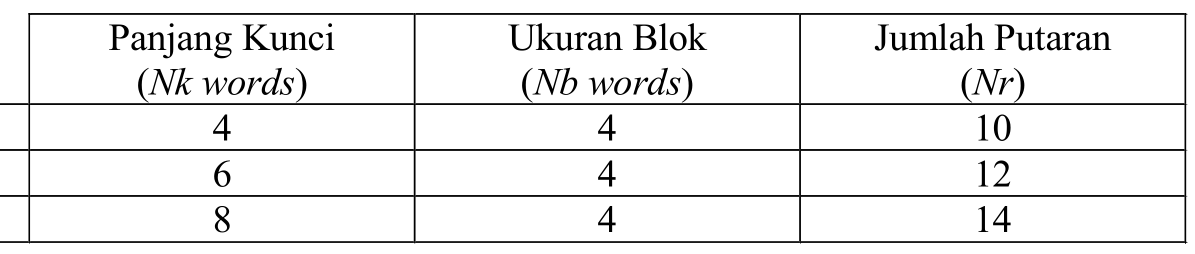
\includegraphics[width=130.62mm,height=70.09mm]{../../images/llm/page_008_img_01.png}%
\end{textblock*}

\end{document}
